\documentclass{beamer}

\usetheme{Madrid}
\usecolortheme{default}

\usepackage{amsmath}
\usepackage{amssymb}
\usepackage{physics}
\usepackage{tikz}

\title{Steady Heat Conduction in a 2D Plate}
\subtitle{Solution of Laplace Equation Using Fourier Series}
\author{Daniel Santiago Carreño Briceño - Finite Element Methods}
\date{}

\begin{document}

%------------------------------------------------
\frame{\titlepage}

%------------------------------------------------
\begin{frame}{Physical Problem}
We study steady heat conduction in a rectangular plate.

\begin{itemize}
\item No internal heat generation
\item Steady state
\item Constant thermal conductivity
\end{itemize}

\vspace{0.5cm}

Governing equation:

\[
\nabla^2 T = 0
\]

This is the \textbf{Laplace equation}.
\end{frame}

%------------------------------------------------
\begin{frame}{Geometry and Boundary Conditions}

\centering
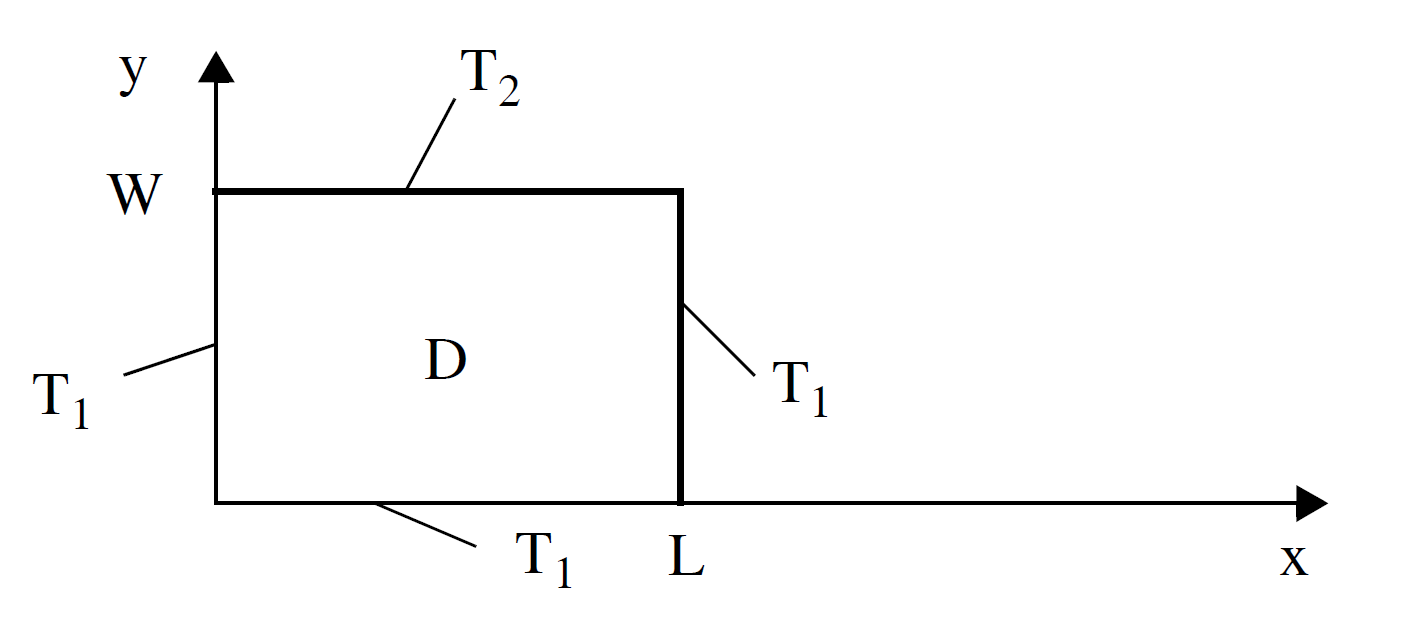
\includegraphics[width=0.7\textwidth]{geometry.png}

\vspace{0.3cm}

Boundary conditions:

\[
\begin{aligned}
T(0,y)&=0\\
T(L,y)&=0\\
T(x,0)&=0\\
T(x,W)&=1
\end{aligned}
\]

\end{frame}

%------------------------------------------------
\begin{frame}{Laplace Equation}

For steady conduction:

\[
\frac{\partial^2 T}{\partial x^2}
+
\frac{\partial^2 T}{\partial y^2}
=0
\]

We solve using:

\begin{block}{Method}
Separation of variables
\end{block}

Assume:

\[
T(x,y)=X(x)Y(y)
\]

\end{frame}

%------------------------------------------------
\begin{frame}{Separation of Variables}

Substituting:

\[
X''Y + XY'' = 0
\]

Divide by $XY$:

\[
\frac{X''}{X} = -\frac{Y''}{Y}=\lambda
\]

We obtain two ODEs:

\[
X''+\lambda X=0
\]

\[
Y''-\lambda Y=0
\]

\end{frame}

%------------------------------------------------
\begin{frame}{Solution in $x$ Direction}

Boundary conditions:

\[
T(0,y)=T(L,y)=0
\]

Thus:

\[
X_n(x)=\sin\left(\frac{n\pi x}{L}\right)
\]

Eigenvalues:

\[
\lambda_n=\left(\frac{n\pi}{L}\right)^2
\]

\end{frame}

%------------------------------------------------
\begin{frame}{Solution in $y$ Direction}

We solve:

\[
Y''-\left(\frac{n\pi}{L}\right)^2Y=0
\]

General solution:

\[
Y_n(y)=A_n e^{n\pi y/L}+B_n e^{-n\pi y/L}
\]

Using hyperbolic functions:

\[
Y_n(y)=C_n\sinh\left(\frac{n\pi y}{L}\right)
\]

because:

\[
T(x,0)=0
\]

\end{frame}

%------------------------------------------------
\begin{frame}{General Solution}

Combining solutions:

\[
T(x,y)=
\sum_{n=1}^{\infty}
C_n
\sin\left(\frac{n\pi x}{L}\right)
\sinh\left(\frac{n\pi y}{L}\right)
\]

Unknown coefficients $C_n$ come from the last boundary condition.

\end{frame}

%------------------------------------------------
\begin{frame}{Applying the Top Boundary}

Boundary:

\[
T(x,W)=1
\]

Therefore:

\[
1=
\sum_{n=1}^{\infty}
C_n
\sinh\left(\frac{n\pi W}{L}\right)
\sin\left(\frac{n\pi x}{L}\right)
\]

We must expand the constant function using a Fourier sine series.

\end{frame}

%------------------------------------------------
\begin{frame}{Fourier Sine Expansion}

We express:

\[
1=\sum_{n=1}^{\infty} A_n
\sin\left(\frac{n\pi x}{L}\right)
\]

Coefficient formula:

\[
A_n=
\frac{2}{L}
\int_0^L
\sin\left(\frac{n\pi x}{L}\right)\,dx
\]

\end{frame}

%------------------------------------------------
\begin{frame}{Computing the Integral}

\[
A_n=
\frac{2}{L}
\left[
-\frac{L}{n\pi}
\cos\left(\frac{n\pi x}{L}\right)
\right]_0^L
\]

\[
A_n=
\frac{2}{n\pi}
\left(1-(-1)^n\right)
\]

Important result:

\begin{itemize}
\item Even $n$ → coefficient = 0
\item Only odd modes survive
\end{itemize}

\end{frame}

%------------------------------------------------
\begin{frame}{Determining $C_n$}

Comparing both expansions:

\[
A_n=
C_n\sinh\left(\frac{n\pi W}{L}\right)
\]

Thus:

\[
C_n=
\frac{2(1-(-1)^n)}
{n\pi\sinh(n\pi W/L)}
\]

\end{frame}

%------------------------------------------------
\begin{frame}{Final Temperature Distribution}

\[
T(x,y)=
\sum_{n=1}^{\infty}
\frac{2(1-(-1)^n)}
{n\pi\sinh(n\pi W/L)}
\sin\left(\frac{n\pi x}{L}\right)
\sinh\left(\frac{n\pi y}{L}\right)
\]

This is the analytical solution of the 2D steady heat conduction problem.

\end{frame}

%------------------------------------------------
\begin{frame}{Physical Interpretation}

\begin{itemize}
\item Each term represents a thermal mode
\item Higher modes decay faster inside the plate
\item Heat diffuses smoothly from the hot boundary
\item Solution satisfies all boundary conditions simultaneously
\end{itemize}

\end{frame}

%------------------------------------------------
\begin{frame}{Connection to Finite Elements}

Why is this important?

\begin{itemize}
\item Analytical benchmark solution
\item Used to validate FEM implementations
\item Shows eigenfunction basis idea
\item FEM approximates this infinite expansion numerically
\end{itemize}

\end{frame}

%------------------------------------------------
%------------------------------------------------
\begin{frame}{References}
    \footnotesize
    
    \begin{thebibliography}{99}
    
    \bibitem{}
    Torrén, P., et al. (Year). \textit{Transferencia de calor}. Paraninfo.
    
    \bibitem{}
    Incropera, F. P., \& DeWitt, D. P. (2007). 
    \textit{Fundamentals of heat and mass transfer} (Spanish ed.). 
    John Wiley \& Sons.
    
    \bibitem{}
    Universidad de Zaragoza. (Year). 
    \textit{Transferencia de calor} (Cap. 3, §3.1: Métodos analíticos en 2D).
    
    \bibitem{}
    Reddy, J. N. (2019). 
    \textit{An introduction to the finite element method}. 
    McGraw–Hill Education.
    
    \bibitem{}
    Zienkiewicz, O. C., Taylor, R. L., \& Zhu, J. Z. (2013). 
    \textit{The finite element method: Its basis and fundamentals}. 
    Butterworth-Heinemann.
    
    \bibitem{}
    Yakhot, V., \& Orszag, S. A. (1986). 
    Renormalization group analysis of turbulence. 
    \textit{Journal of Scientific Computing}.
    
    \bibitem{}
    Batchelor, G. K. (2000). 
    \textit{An introduction to fluid dynamics}. 
    Cambridge University Press.
    
    \bibitem{}
    Universidad de Santiago; Universidad Nacional. (Year). 
    \textit{Notas de curso sobre ecuaciones de Laplace y Poisson en transferencia de calor}.
    
    \end{thebibliography}
    
    \end{frame}
    %------------------------------------------------

\end{document}